\chapter{Introduction}

The later part of the past decade has seen a tremendous increase in the research of Internet of Things (IoT) devices mostly geared towards energy efficiency.
This is in part, due to the fact that IoT devices have an underlining positive factor of having to save energy usage and hence must be design as not excessively use energy in itself.
Not only do these interconnected devices provide comfort but have also become critical parts of our daily lives: saving lives, expediting interactions and transactions.
Another factor that fueled the advancement in the research of energy efficient IoT devices is the enormous progress made in the field of Machine learning specifically Reinforcement learning.\\\\
Maximizing a numerical reward signal by learning which actions to take in a given situation is what Reinforcement learning is about.
The actions to take by the learning agent pertaining to various situations are not preprogrammed into the learner, but instead this is discovered by taking the actions that maximize the reward margin\cite{Sutton&Barto}. This works in the cycle of sense-action-goals and learning is from immediate interactions with the environment.\\\\
The APT-MAC protocol, which is the focus of this paper, seeks to solve the problem of the reliance on battery.
The protocol utilizes the Multi-Arm Bandit algorithm, a reinforcement learning algorithm, in tandem with Radio-frequency identification (RFID) signals to enable battery-free communication of wireless devices\cite{Maselli}.\\\\
The aim of this work is to simulate the APT-MAC protocol in NS3 and in comparison to the static TDMA protocol.

\section{The Protocols}
Even though the quality of a network service is a cooperative effort of all the stack of communication protocols, the MAC layer is of a peculiar importance as it handles the sharing of the medium on which all other upper-layered protocols depend.
MAC protocols do not only solve the problem of medium sharing, hence, support for reliable communication but also, in Wireless Sensor Networks, control of energy utilization, achieve through duty cycling and retransmissions or transmission power control\cite{Yigitel&Durmaz&Ersoy}.\\\\
In wireless sensor network, the MAC protocols are broadly classified into contention-based MAC protocols and scheduled-based MAC protocols depending on how he medium is accessed\cite{Pal&Chatterjee}.\\\\
The medium in a contention-base MAC protocol is accessed by all the nodes and, as the name suggests, the nodes contend for access to the medium this may result in collision hence, to prevent collision access to the medium is negotiated through probabilistic coordination.
A sending node listens to shared medium before sending, if the medium is busy, sending is halted for a specified period of time before retrying.
Examples of contention-based MAC protocols used in wireless sensor network are ALOHA (Additive Link On-line Hawaii System)and CSMA (Carrier Sense Multiple Access)\cite{Tanenbaum&Wetherall}.\\\\
Nodes' medium access in a schedule-based MAC protocol is split into either frequency, Frequency Division Multiple Access, or time, that is, Time Division Multiple Access, or orthogonal pseudo - noise codes (Code Division Multiple Access).
Collision is prevent in the medium by making different nodes access the medium in their designated time or frequency and hence not interfering with each other.\\\\
This section deals with the description of the protocol: APT-MAC and Time Division Multiple Access (TDMA).

\subsection{TDMA}
In TDMA, the total duration of communication is divided into fixed number of time slots.
Time slots are configured into time-frames that are repeated periodically.
Each node is allocated a time slot in a time-frame and is allowed to only transmit in that time slot.
The TDMA frame structure has extra overhead; preamble and trail bits, added to the information message or bits.
Time slots are what make up the information bits/message.
Figure \ref{fig:frame_structure} shows the details of the frame structure.\newline
\textbf{Preamble:} contains the address and synchronization information of the base (sink) node and the identification information of the other nodes.\newline
\textbf{Guard time:} necessary to prevent time-drifting over time.\newline
\textbf{Trail bit:} for error detection in the form of checksum or cyclic redundancy check.\newline
\begin{figure}[h]
    \centering
    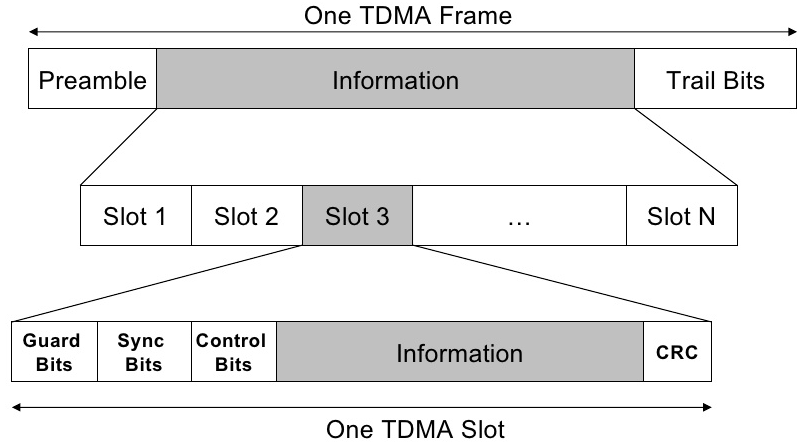
\includegraphics[scale=0.5]{frame_structure}
    \caption{Frame Structure}
    \label{fig:frame_structure}
\end{figure} \newline
The inadequacies of TDMA, chief among them with respect to the aim of the referenced paper \cite{Maselli}, is static slot assignment.
The slots are assigned before transmission and does not change whatsoever during the transmission process, this does not serve the purpose of a protocol that is needed to scale according to the transmission requirements of the nodes.

\subsection{APT-MAC}
APT-MAC protocol is a zero configuration - manual configuration not needed - mac protocol.
Reinforcement learning is utilized to learn the required rate of transmission of each active node and continually update the transmission requirements of nodes.
An overview of the reinforcement learning algorithm is given, followed by how it is used the APT-MAC protocol.
\subsubsection{Multi-Arm Bandit}
    
\subsubsection{APT-MAC protocol overview}
The "battery-freeness" of the protocol is as a result of the use of sensor-augmented RFID tags.

During initialization, the reader sends discovery queries to all nodes and each is assigned a unique identification.
In querying tags in such a way as to minimize the difference between the sensor's data generation time and the time of delivery of data to the reader, the Multi-Arm Bandit, describe above, is used.
The reader, agent in this case, queries each node - set of actions - and can be in one of two states: querying or ready to query.
Expected reward is calculated with the formula \ref{expected_reward} with the expected reward of each action stored in vector $Q$.
\begin{equation}
    Q(a_i)(n+1) = Q(a_i)(n)+\alpha(Reward - Q(a_i)(n))
    \label{expected_reward}
\end{equation}
$n$ is the time slot of the query, $a_i$ is the action of querying tag $i$ and $\alpha$ is the learning rate.\newline
A more detailed explanation of the protocol, such as the learning rate parameter and theevaluation of the $Reward$ can be found in \cite{Maselli}.
